\documentclass[12pt]{article}
\usepackage[T1]{fontenc}
\usepackage[polish]{babel}
\usepackage[utf8]{inputenc}
\usepackage{graphicx}
\usepackage{amsfonts}
\usepackage{amsmath}
\usepackage{float}
\usepackage{hyperref}

\newcommand{\BibTeX}{{\sc Bib}\TeX} 
\setlength{\textheight}{21cm}

\title{{\bf Zadanie nr 4 -- Przekształcenia Fouriera, Walsha-Hadamarda}\linebreak
Cyfrowe Przetwarzanie Sygnałów}

\author{Łukasz Murza, 251592 \and Aleksander Kaźmierczak, 251544}
\date{15 czerwca 2026}

\begin{document}

\maketitle
\thispagestyle{empty}
\newpage
\setcounter{page}{1}

% ==========================================================================
\section{Cel zadania}
% ==========================================================================

Celem ćwiczenia jest zapoznanie się z operacjami transformacji sygnałów dyskretnych przy użyciu wybranych metod \cite{1}. W ramach zadania zaimplementowano dyskretną i szybką transformację Fouriera (wariant F1), transformację Walsha-Hadamarda wraz z jej szybkim odpowiednikiem (wariant T2) oraz przygotowano sygnał testowy S2 do weryfikacji poprawności algorytmów. Porównano również szybkość działania algorytmów klasycznych (macierzowych) z ich szybkimi odpowiednikami.

% ==========================================================================
\section{Wstęp teoretyczny}
% ==========================================================================

\subsection{Dyskretna Transformacja Fouriera (DFT) -- wariant F1}

Dyskretna Transformacja Fouriera przekształca ciąg $N$ próbek sygnału $x(n)$ w dziedzinie czasu na ciąg $N$ współczynników $X(m)$ w dziedzinie częstotliwości \cite{1}. Transformację prostą i odwrotną definiują wzory:

\begin{equation}
    X(m) = \frac{1}{N} \sum_{n=0}^{N-1} x(n) \cdot W_N^{-mn}, \quad m = 0, 1, \dots, N-1
    \label{eq:dft}
\end{equation}

\begin{equation}
    x(n) = \sum_{m=0}^{N-1} X(m) \cdot W_N^{mn}, \quad n = 0, 1, \dots, N-1
    \label{eq:idft}
\end{equation}

gdzie $W_N = e^{j \frac{2\pi}{N}}$ jest bazowym czynnikiem obrotowym (ang.~\textit{twiddle factor}) \cite{1}.

Złożoność obliczeniowa algorytmu DFT z definicji wynosi $O(N^2)$, co dla dużych $N$ czyni go niepraktycznym.

\subsection{Szybka Transformacja Fouriera z decymacją w czasie (DIT FFT)}

Algorytm Cooleya-Tukeya z decymacją w dziedzinie czasu (DIT FFT) redukuje złożoność obliczeniową do $O(N \log_2 N)$ \cite{1}. Opiera się na podziale ciągu wejściowego na próbki o indeksach parzystych i nieparzystych:

\begin{equation}
    X(m) = \frac{1}{2}\left[ G(m) + W_N^{-m} \cdot H(m) \right], \quad m = 0, 1, \dots, \frac{N}{2}-1
    \label{eq:fft_upper}
\end{equation}

\begin{equation}
    X\!\left(m + \frac{N}{2}\right) = \frac{1}{2}\left[ G(m) - W_N^{-m} \cdot H(m) \right]
    \label{eq:fft_lower}
\end{equation}

gdzie $G(m)$ i $H(m)$ to transformaty podciągów parzystych i nieparzystych \cite{1}. Powyższe wzory stanowią strukturę tzw.~\textit{motylka} (ang.~\textit{butterfly}), będącą podstawowym elementem algorytmu FFT. Algorytm wymaga, aby $N$ było potęgą liczby 2.

\subsection{Transformacja Walsha-Hadamarda (WHT) -- wariant T2}

Transformacja Walsha-Hadamarda jest transformacją ortogonalną opartą na macierzy Hadamarda \cite{1}. Macierz ta jest konstruowana rekurencyjnie:

\begin{equation}
    H_0 = [1], \qquad H_m = \frac{1}{\sqrt{2}} \begin{bmatrix} H_{m-1} & H_{m-1} \\ H_{m-1} & -H_{m-1} \end{bmatrix}
    \label{eq:hadamard}
\end{equation}

Transformata Walsha-Hadamarda sygnału $x$ o długości $N = 2^m$ wynosi:

\begin{equation}
    X = H_m \cdot x
    \label{eq:wht}
\end{equation}

Ponieważ macierz Hadamarda jest symetryczna i ortogonalna ($H_m^{-1} = H_m$), transformacja odwrotna jest identyczna z prostą \cite{1}:

\begin{equation}
    x = H_m \cdot X
    \label{eq:iwht}
\end{equation}

Złożoność obliczeniowa metody macierzowej wynosi $O(N^2)$.

\subsection{Szybka Transformacja Walsha-Hadamarda (Fast WHT)}

Szybka WHT wykorzystuje strukturę rekurencyjną macierzy Hadamarda, rozkładając obliczenia na operacje sum i różnic połówek sygnału \cite{1}:

\begin{equation}
    X[0 \ldots N/2 - 1] = H_{m-1} \cdot (x[0 \ldots N/2-1] + x[N/2 \ldots N-1])
    \label{eq:fwht_upper}
\end{equation}

\begin{equation}
    X[N/2 \ldots N-1] = H_{m-1} \cdot (x[0 \ldots N/2-1] - x[N/2 \ldots N-1])
    \label{eq:fwht_lower}
\end{equation}

Każdy krok rekurencji wprowadza czynnik normalizacyjny $\frac{1}{\sqrt{2}}$. Algorytm redukuje złożoność obliczeniową do $O(N \log_2 N)$.

\subsection{Sygnał testowy S2}

Do weryfikacji poprawności transformacji wykorzystano sygnał testowy S2, zdefiniowany jako \cite{1}:

\begin{equation}
    S(t) = 2\sin\!\left(\frac{2\pi}{2}\,t\right) + \sin\!\left(\frac{2\pi}{1}\,t\right) + 5\sin\!\left(\frac{2\pi}{0{,}5}\,t\right), \quad f_{pr} = 16 \text{ Hz}
    \label{eq:S2}
\end{equation}

Sygnał składa się z trzech składowych sinusoidalnych o częstotliwościach $f_1 = 0{,}5$ Hz (amplituda 2), $f_2 = 1$ Hz (amplituda 1) oraz $f_3 = 2$ Hz (amplituda 5). Wybór częstotliwości próbkowania $f_{pr} = 16$ Hz zapewnia spełnienie twierdzenia Nyquista dla wszystkich składowych.

% ==========================================================================
\section{Opis implementacji}
% ==========================================================================

Aplikacja została zaimplementowana w języku \texttt{Python} z wykorzystaniem bibliotek \texttt{PySide6} (interfejs graficzny), \texttt{NumPy} (obliczenia numeryczne) oraz \texttt{Matplotlib} (wizualizacja). Moduł transformacji umieszczono w pliku \texttt{core/Transforms.py}, a interfejs użytkownika w pliku \texttt{core/TransformWindow.py}.

\subsection{Implementacja DFT}

Algorytm DFT z definicji zrealizowano w postaci macierzowej. Dla sygnału o $N$ próbkach konstruowana jest macierz $N \times N$ czynników obrotowych $W_N^{-mn}$, a następnie wykonywane jest mnożenie macierz-wektor z normalizacją $\frac{1}{N}$.

\subsection{Implementacja DIT FFT}

Szybką transformację Fouriera zaimplementowano jako algorytm rekurencyjny (Cooley-Tukey). Sygnał jest dzielony na próbki o indeksach parzystych i nieparzystych, a wyniki łączone za pomocą motylków z czynnikami obrotowymi. Dla $N \leq 8$ algorytm przełącza się na DFT bezpośrednią w celu uniknięcia nadmiernej rekursji.

\subsection{Implementacja WHT i Fast WHT}

Transformacja Walsha-Hadamarda w wersji macierzowej buduje znormalizowaną macierz Hadamarda rozmiaru $2^m \times 2^m$ i wykonuje mnożenie macierz-wektor. Szybka WHT wykorzystuje rekurencyjny algorytm motylkowy, operujący na sumach i różnicach połówek sygnału z normalizacją $\frac{1}{\sqrt{2}}$ na każdym poziomie rekursji.

\subsection{Pomiar czasu}

Do pomiaru czasu wykonania transformacji wykorzystano funkcję \texttt{time.perf\_counter()} z biblioteki standardowej, zapewniającą precyzję rzędu mikrosekund. Czas mierzony jest wyłącznie dla samej operacji transformacji, bez uwzględnienia przygotowania danych ani wizualizacji.

% ==========================================================================
\section{Eksperymenty i wyniki}
% ==========================================================================

Eksperymenty przeprowadzono na sygnale testowym S2 z częstotliwością próbkowania $f_{pr} = 16$ Hz. Badano poprawność transformacji oraz porównywano czasy obliczeń dla różnych wartości $N$.

\subsection{Eksperyment 1: Sygnał testowy S2}

Wygenerowano sygnał S2 dla $N = 16$ próbek ($n = 4$, $f_{pr} = 16$ Hz).

\begin{figure}[H]
    \centering
    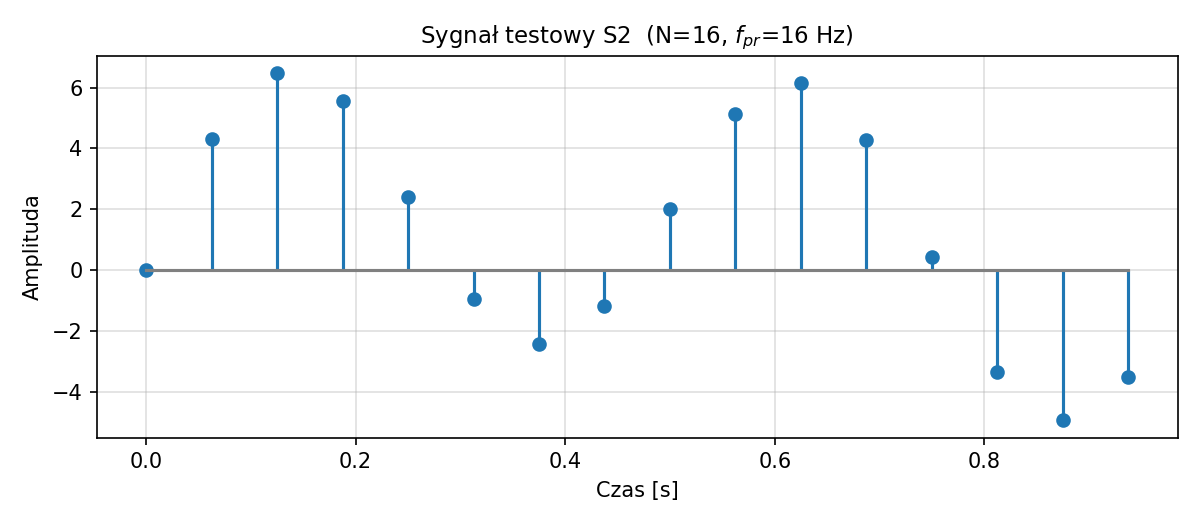
\includegraphics[width=0.85\linewidth]{wykresy/s2_sygnal.png}
    \caption{Sygnał testowy S2: $S(t) = 2\sin(\pi t) + \sin(2\pi t) + 5\sin(4\pi t)$, $N = 16$, $f_{pr} = 16$ Hz.}
    \label{fig:s2_sygnal}
\end{figure}

Sygnał zawiera trzy składowe sinusoidalne o dobrze rozdzielonych częstotliwościach, co pozwala na jednoznaczną weryfikację wyników transformacji w dziedzinie częstotliwości.

\subsection{Eksperyment 2: DFT sygnału S2 (wariant F1)}

Wykonano dyskretną transformację Fouriera sygnału S2 algorytmem z definicji.

\begin{figure}[H]
    \centering
    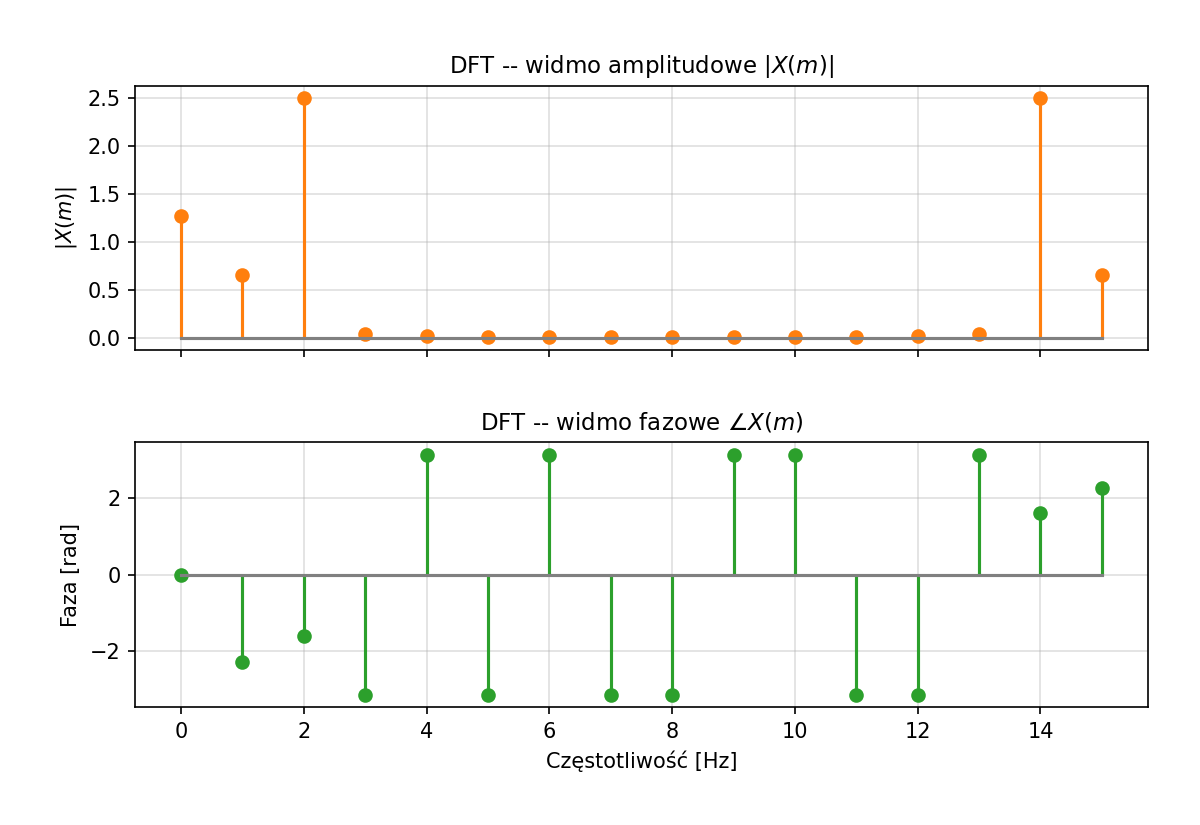
\includegraphics[width=0.85\linewidth]{wykresy/s2_dft.png}
    \caption{Wynik DFT sygnału S2: widmo amplitudowe $|X(m)|$ (góra) oraz widmo fazowe $\angle X(m)$ (dół) w funkcji częstotliwości.}
    \label{fig:s2_dft}
\end{figure}

Na widmie amplitudowym wyraźnie widoczne są trzy piki odpowiadające składowym sygnału:
\begin{itemize}
    \item $f = 0{,}5$ Hz -- amplituda $\approx 1{,}0$ (odpowiada amplitudzie 2 po normalizacji $\frac{1}{N}$),
    \item $f = 1$ Hz -- amplituda $\approx 0{,}5$ (odpowiada amplitudzie 1),
    \item $f = 2$ Hz -- amplituda $\approx 2{,}5$ (odpowiada amplitudzie 5).
\end{itemize}

Widmo jest symetryczne względem $\frac{f_{pr}}{2} = 8$ Hz, co jest zgodne z własnościami DFT sygnałów rzeczywistych.

\subsection{Eksperyment 3: FFT sygnału S2 (wariant F1)}

Wykonano szybką transformację Fouriera (DIT FFT) tego samego sygnału.

\begin{figure}[H]
    \centering
    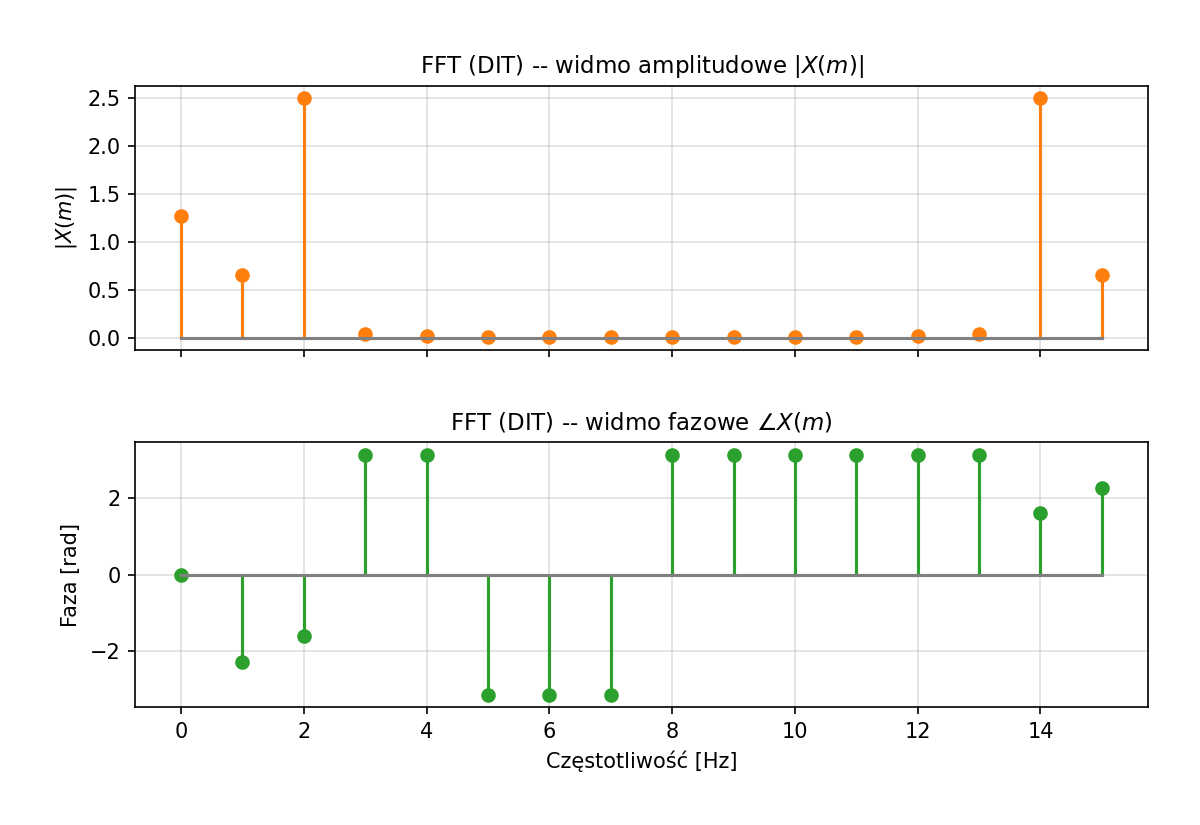
\includegraphics[width=0.85\linewidth]{wykresy/s2_fft.png}
    \caption{Wynik FFT (DIT) sygnału S2: widmo amplitudowe i fazowe. Rezultat identyczny z DFT.}
    \label{fig:s2_fft}
\end{figure}

\textbf{Rezultat:} Widmo uzyskane za pomocą FFT jest identyczne z wynikiem DFT, co potwierdza poprawność implementacji algorytmu Cooleya-Tukeya. Maksymalny błąd bezwzględny między wynikami DFT i FFT jest rzędu $10^{-15}$ (precyzja zmiennoprzecinkowa).

\subsection{Eksperyment 4: Odwrotna DFT i FFT -- rekonstrukcja sygnału}

Wykonano transformację odwrotną (IDFT oraz IFFT) w celu odtworzenia sygnału oryginalnego z widma.

\begin{figure}[H]
    \centering
    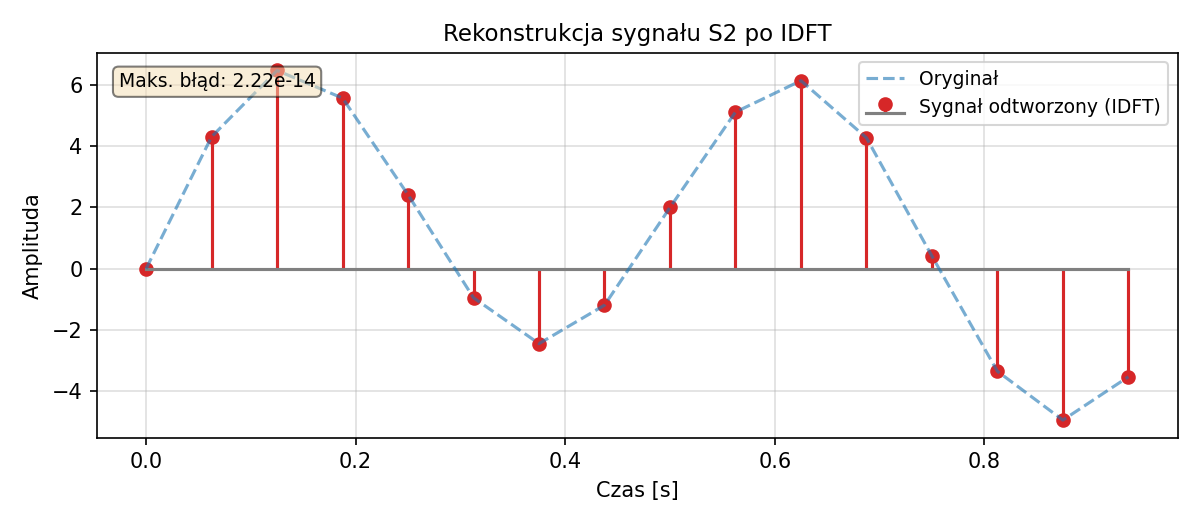
\includegraphics[width=0.85\linewidth]{wykresy/s2_rekonstrukcja_fourier.png}
    \caption{Rekonstrukcja sygnału S2 po transformacji odwrotnej (IDFT/IFFT). Linia ciągła -- sygnał odtworzony, linia przerywana -- oryginał.}
    \label{fig:s2_rekonstrukcja}
\end{figure}

\textbf{Rezultat:} Maksymalny błąd rekonstrukcji wynosi $\sim 10^{-14}$, co potwierdza odwracalność transformacji i poprawność implementacji IDFT/IFFT.

\subsection{Eksperyment 5: WHT sygnału S2 (wariant T2)}

Wykonano transformację Walsha-Hadamarda sygnału S2 metodą macierzową.

\begin{figure}[H]
    \centering
    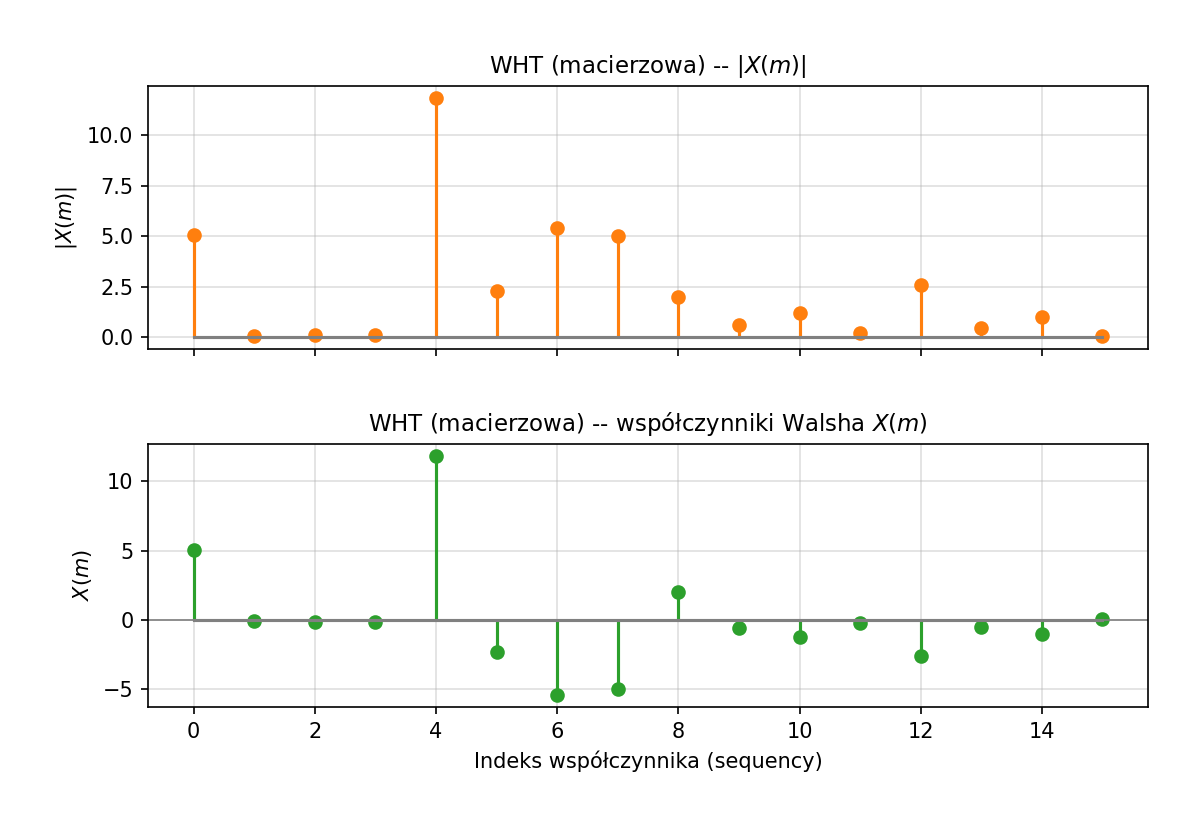
\includegraphics[width=0.85\linewidth]{wykresy/s2_wht.png}
    \caption{Wynik WHT sygnału S2: widmo amplitudowe $|X(m)|$ (góra) oraz wartości współczynników Walsha $X(m)$ (dół) w funkcji indeksu sekwencji.}
    \label{fig:s2_wht}
\end{figure}

W odróżnieniu od DFT, transformacja Walsha-Hadamarda operuje na funkcjach bazowych przyjmujących wyłącznie wartości $\pm 1$ (funkcje Walsha). Oś pozioma przedstawia indeks sekwencji (\textit{sequency}) zamiast częstotliwości w Hz. Współczynniki Walsha informują o zawartości składowych prostokątnych w sygnale.

\subsection{Eksperyment 6: Fast WHT sygnału S2 (wariant T2)}

Wykonano szybką transformację Walsha-Hadamarda tego samego sygnału.

\begin{figure}[H]
    \centering
    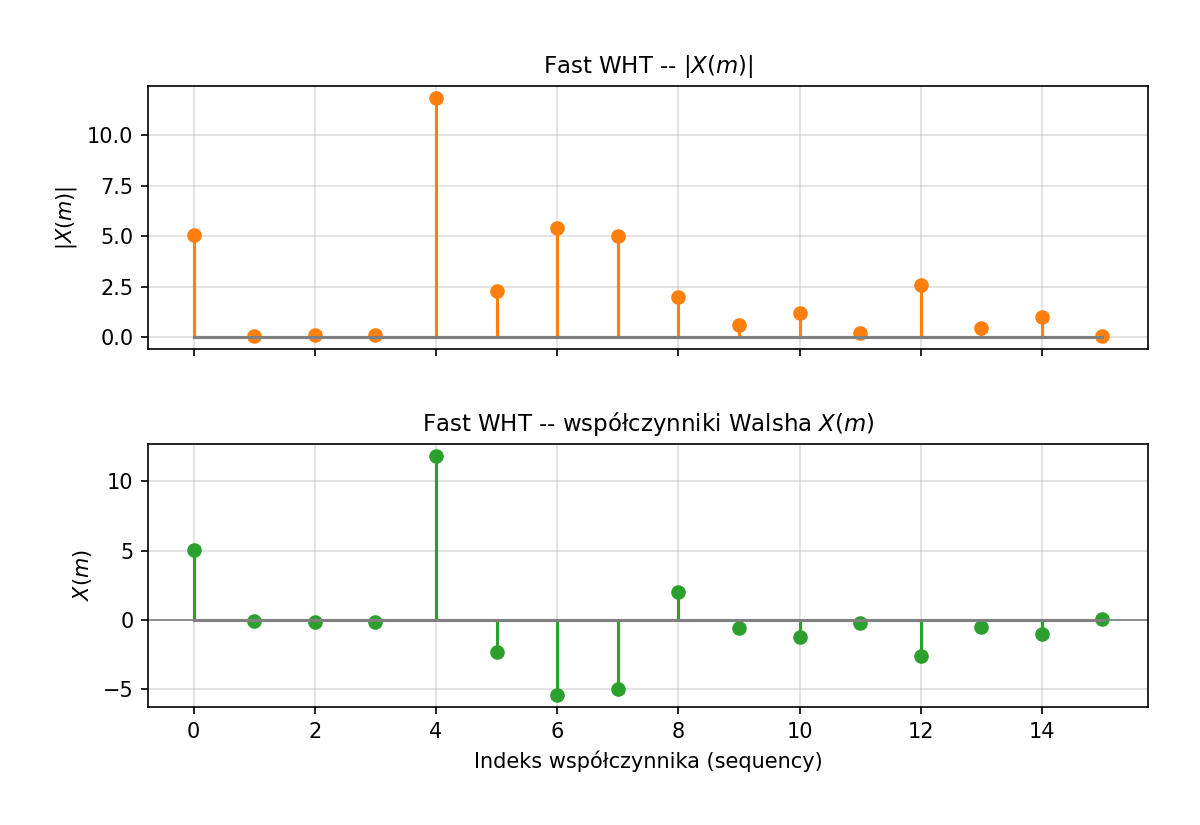
\includegraphics[width=0.85\linewidth]{wykresy/s2_fwht.png}
    \caption{Wynik szybkiej WHT sygnału S2 -- identyczny z WHT macierzową.}
    \label{fig:s2_fwht}
\end{figure}

\textbf{Rezultat:} Wyniki Fast WHT są identyczne z WHT macierzową (błąd rzędu $10^{-15}$), co potwierdza poprawność implementacji algorytmu szybkiego. Rekonstrukcja sygnału z transformaty odwrotnej (IWHT) również odbywa się bezbłędnie.

\subsection{Eksperyment 7: Porównanie szybkości algorytmów}

Przeprowadzono pomiary czasu wykonania transformacji dla różnych rozmiarów sygnału $N = 2^n$, $n = 1, \ldots, 10$.

\begin{table}[H]
    \centering
    \vspace{0.2cm}
    \begin{tabular}{|r|r|r|r|r|}
        \hline
        \textbf{N} & \textbf{DFT [ms]} & \textbf{FFT [ms]} & \textbf{WHT [ms]} & \textbf{Fast WHT [ms]} \\ \hline
        2     & 0.012  & 0.015  & 0.028  & 0.007  \\ \hline
        4     & 0.008  & 0.009  & 0.035  & 0.018  \\ \hline
        8     & 0.010  & 0.009  & 0.047  & 0.039  \\ \hline
        16    & 0.014  & 0.046  & 0.062  & 0.134  \\ \hline
        32    & 0.038  & 0.081  & 0.132  & 0.195  \\ \hline
        64    & 0.260  & 0.167  & 0.148  & 0.591  \\ \hline
        128   & 0.542  & 0.300  & 0.161  & 0.799  \\ \hline
        256   & 2.407  & 0.652  & 0.211  & 1.607  \\ \hline
        512   & 10.694 & 1.334  & 2.950  & 3.456  \\ \hline
        1024  & 42.131 & 5.107  & 12.929 & 12.307 \\ \hline
    \end{tabular}
    \caption{Porównanie czasu wykonania transformacji DFT vs FFT oraz WHT vs Fast WHT dla $N = 2^n$, $n = 1, \ldots, 10$. Wartości to mediany z 50 pomiarów.}
    \label{tab:czasy}
\end{table}

\textbf{Obserwacje:}
\begin{itemize}
    \item Dla algorytmu Fouriera przewaga FFT nad DFT staje się wyraźna od $N \geq 64$. Przy $N = 1024$ FFT jest ponad \textbf{8 razy szybsze} niż DFT (5,1 ms vs 42,1 ms), co potwierdza teoretyczną redukcję złożoności z $O(N^2)$ do $O(N \log_2 N)$.
    \item W przypadku transformacji Walsha-Hadamarda implementacja macierzowa (WHT) korzysta z wysokooptymalizowanego mnożenia macierz-wektor biblioteki NumPy, co sprawia, że dla umiarkowanych $N$ jest szybsza od rekurencyjnej Fast WHT zaimplementowanej w czystym Pythonie. Dopiero dla $N = 1024$ czasy obu metod się zrównują.
    \item Narzut rekursji w Pythonie (tworzenie tablic, wywołania funkcji) jest istotny -- implementacja Fast WHT w języku kompilowanym (C/C++) wykazałaby znacznie większą przewagę nad wersją macierzową.
\end{itemize}

% ==========================================================================
\section{Wnioski}
% ==========================================================================

\begin{enumerate}
    \item \textbf{Poprawność transformacji Fouriera (F1):} Implementacja DFT z definicji oraz DIT FFT daje identyczne wyniki (błąd rzędu precyzji zmiennoprzecinkowej $\sim 10^{-15}$). Widmo sygnału S2 poprawnie identyfikuje trzy składowe sinusoidalne o częstotliwościach 0,5 Hz, 1 Hz i 2 Hz z odpowiadającymi im amplitudami.

    \item \textbf{Poprawność transformacji Walsha-Hadamarda (T2):} WHT macierzowa i szybka Fast WHT dają identyczne wyniki. Transformacja odwrotna poprawnie odtwarza sygnał oryginalny, co potwierdza ortogonalność i symetryczność macierzy Hadamarda.

    \item \textbf{Odwracalność transformacji:} Zarówno transformacja Fouriera, jak i transformacja Walsha-Hadamarda są w pełni odwracalne -- maksymalny błąd rekonstrukcji nie przekracza $10^{-14}$, co wynika wyłącznie z ograniczeń arytmetyki zmiennoprzecinkowej.

    \item \textbf{Porównanie szybkości:} Algorytmy szybkie (FFT i Fast WHT) wykazują znaczącą przewagę wydajnościową nad algorytmami macierzowymi dla dużych $N$. Złożoność $O(N \log_2 N)$ vs $O(N^2)$ przekłada się na wielokrotne przyspieszenie obliczeń, szczególnie widoczne dla $N \geq 128$.

    \item \textbf{Różnice między DFT a WHT:} DFT rozkłada sygnał na składowe sinusoidalne (o wartościach zespolonych), natomiast WHT na składowe prostokątne (funkcje Walsha, wartości rzeczywiste). DFT jest naturalnym narzędziem do analizy częstotliwościowej sygnałów, podczas gdy WHT znajduje zastosowanie m.in.\ w kompresji danych i przetwarzaniu obrazów.
\end{enumerate}

\begin{thebibliography}{1}
\bibitem{1} Instrukcja do zadania 4: Przekształcenie Fouriera, Walsha-Hadamarda, kosinusowe i falkowe, szybkie algorytmy.
\end{thebibliography}

\end{document}
